% Fragment for a new experiment-3 section. Not a standalone document.
% Do not compile this file alone, and do not replace fig:exp3-ablation.
% Suggested label fig:exp3-scale is not yet agreed.
% Graphic: recovery/e3/e3-scale.pdf
% Drawn at 178 mm by 136 mm. 178 mm is the double-column measure.
% \includegraphics[width=178mm] matches that width 1:1.

\begin{figure*}[t]
  \centering
  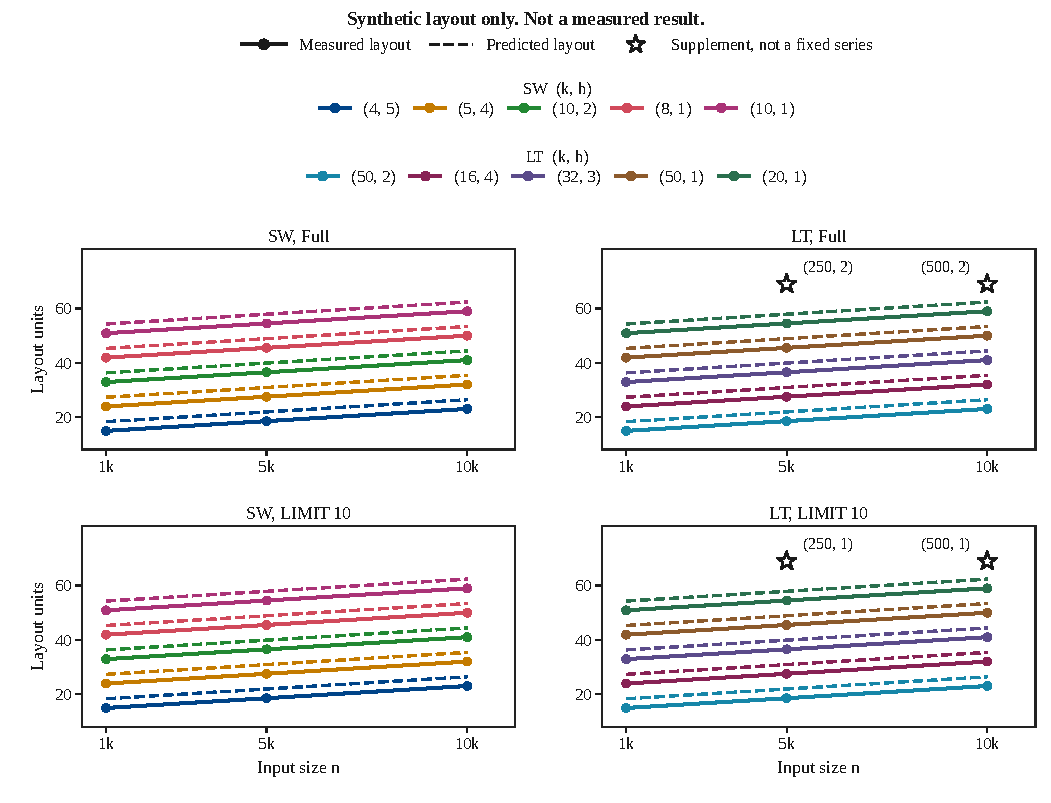
\includegraphics[width=178mm]{e3-scale.pdf}
  \caption{Synthetic layout for the fixed-$(k,h)$ scale figure, not a measured result.
  The contract names Qwen3.5-9B and one DL20 query; no run produced these heights.
  Input size $n$ is linear at 1k, 5k, and 10k. A logarithmic axis was not specified.
  Each color is one confirmed pair and is the same in the Full and LIMIT~10 panels of that family.
  A solid line with filled circles stands in for a measurement.
  A dashed line stands in for a prediction: the same scaffold plus a constant offset, not a model error.
  Vertical order follows the confirmed list and is not a ranking.
  Open stars are the four LT supplements and are not joined to the five series.
  Full uses $(250,2)$ at 5k and $(500,2)$ at 10k.
  LIMIT~10 uses $(250,1)$ at 5k and $(500,1)$ at 10k.
  Those stars are not per-size optima.
  The vertical unit is a layout unit, not tokens and not a cost.
  Cache off/on is not split, and per-size best $(k,h)$ are omitted.}
  \label{fig:exp3-scale}
\end{figure*}
